%-------------------------------------------------------------------------------
%							PREAMBULE
%-------------------------------------------------------------------------------

\documentclass[xcolor=dvipsnames]{beamer} % dvipsnames gives more built-in colors

\usetheme{Szeged}
\useoutertheme{miniframes} % Alternatively: miniframes, infolines, split, smoothbars, smoothtree, shadow
\useinnertheme{rectangles}

\usepackage{media9}
\usepackage{graphicx}

\usepackage{docmute} % To include multiple files

\usepackage{tikz}
\usetikzlibrary{positioning,shapes,arrows}
\usetikzlibrary{babel}      % Utiliser ce Babel pour eviter les problemes avec les animations TIKX
% \usepackage{csquotes}

\usepackage{iwona}
% \usepackage{lmodern}
% \usepackage[french]{babel}
\graphicspath{ {./Figures/} }
\usepackage[utf8]{inputenc}
\newcommand{\bvec}[1]{\mathbf{#1}} 
\usepackage{amsmath,bm,mathtools}
\usepackage{siunitx}

\usepackage[backend=bibtex,style=authoryear,maxnames=2,natbib=true]{biblatex} % Use the bibtex backend with the authoryear citation style (which resembles APA)
\addbibresource{bibliographie.bib} % The filename of the bibliography
\usepackage[autostyle=true]{csquotes} % Required to generate language-dependent quotes in the bibliography 
\renewcommand*{\bibfont}{\scriptsize} % Pour reduire la taille des references

\usepackage[font=scriptsize]{caption}
\captionsetup{labelformat=empty,labelsep=none}    % Pour retirer le terme figure des titres

\usepackage{booktabs}

\definecolor{UBCblue}{rgb}{0.04706, 0.13725, 0.26667} % UBC Blue (primary)

\definecolor{MyGreen}{RGB}{0, 50, 0}
\definecolor{MyRed}{RGB}{100, 0, 0}

% \usecolortheme[named=UBCblue]{structure}
\usecolortheme[named=MyGreen]{structure} % Sample dvipsnames color
\setbeamercolor{alerted text}{fg=MyRed}
% \definecolor{darkred}{rgb}{0.4,0.5,0}
% \setbeamercolor{titlelike}{parent=structure,bg=yellow!85!orange}


%-------------------------------------------------------------------------------
%							A CUSTOM FOOTLINE
%-------------------------------------------------------------------------------

\makeatletter
\setbeamertemplate{footline}{
	\begin{beamercolorbox}[colsep=1.5pt]{upper separation line foot}
	\end{beamercolorbox}
  \leavevmode%
  \hbox{%
  \begin{beamercolorbox}[wd=.333333\paperwidth,ht=2.25ex,dp=1ex,center]{author in head/foot}%
	% \usebeamerfont{author in head/foot}\insertshortauthor\expandafter\beamer@ifempty\expandafter{\beamer@shortinstitute}{}{~~(\insertshortinstitute)}
	\insertshortauthor
  \end{beamercolorbox}%
  \begin{beamercolorbox}[wd=.333333\paperwidth,ht=2.25ex,dp=1ex,center]{title in head/foot}%
    \usebeamerfont{title in head/foot}\insertshorttitle
  \end{beamercolorbox}%
  \begin{beamercolorbox}[wd=.333333\paperwidth,ht=2.25ex,dp=1ex,right]{date in head/foot}%
    \usebeamerfont{date in head/foot}\insertshortdate{}\hspace*{2em}
    \insertframenumber{} / \inserttotalframenumber\hspace*{2ex} 
  \end{beamercolorbox}}%
  \vskip0pt%

  \begin{beamercolorbox}[colsep=1.5pt]{lower separation line foot}
  \end{beamercolorbox}

}
\makeatother

%-------------------------------------------------------------------------------
%							FIRST TITLE PAGE
%-------------------------------------------------------------------------------

\title[Problème Inverse : Transfert Radiatif et Apprentissage]{Problème Inverse : Transfert Radiatif et Apprentissage}
\date{\today}
\author[Roussel Desmond NZOYEM]{Roussel Desmond NZOYEM}

\institute[Université de Strasbourg]{Université de Strasbourg\\UFR de mathématiques et d'informatque\\Master 1 CSMI}

\begin{document}

\begingroup
\setbeamertemplate{navigation symbols}{}
\setbeamertemplate{headline}{\vspace{0.5cm}%
  \hspace*{0.8cm}%
  
\includegraphics[width=3cm]{LogoUnistra}
  \hfill\raisebox{.2cm}{\normalsize Soutenance de stage}\hfill%
  
\includegraphics[width=2.2cm]{LogoIRMA}
  \hspace*{0.8cm}%
}
\begin{frame}
\maketitle
\end{frame}
\endgroup

%-------------------------------------------------------------------------------
%							SECOND TITLE PAGE
%-------------------------------------------------------------------------------

%------------ Intro Part 1
% - Moi (Nom-prenom-classe)
% - Remerciement des profs, qui ont ausi encadrer le projer
% - Parler du projet

\begingroup  % A new griou whose informations are not cannon., just for convenience

\title[Problème Inverse : Transfert Radiatif et Apprentissage]{Simulation 2D de l’équation du transfert radiatif et reconstruction de la densité par un réseau de neurones}

\author[Roussel Desmond NZOYEM]{Roussel Desmond NZOYEM\\[2mm]{\small \textbf{ \hspace*{0.1mm} Ensignant referent} \hspace*{11mm} \textbf{Maitre de stage} \\ \footnotesize Christophe PRUD'HOMME \hspace*{6mm} Emmanuel FRANCK \\ \hspace*{44.5mm} Laurent NAVORET \\ \hspace*{44.5mm} Vincent VIGON}}

\institute[Université de Strasbourg]{}
\date[\today]{\footnotesize Annee Academique 2019/2020}

\setbeamertemplate{navigation symbols}{}
\setbeamertemplate{headline}{\vspace{0.5cm}%
  \hspace*{0.8cm}%
  
\includegraphics[width=3cm]{LogoUnistra}
  \hfill\raisebox{.6cm}{}\hfill%
  
\includegraphics[width=2.2cm]{LogoIRMA}
  \hspace*{0.8cm}%
}
\begin{frame}
\maketitle
\end{frame}
\endgroup

%-------------------------------------------------------------------------------
%							INCLUDE THE CHAPTERS
%-------------------------------------------------------------------------------

% \documentclass{beamer}
% \usetheme{Szeged}

% \begin{document}


%-------------------------------------------------------------------------------
%							FIRST SECTION
%-------------------------------------------------------------------------------

%------------ Intro Part 2
% - le site de l'IRMA est riche et complet
% - De M.NAVORET et FRANCK vers l'equipe MOCO (leurs travaux, etc..):
% - l'equipe probabilite

\section{Introduction}    % L'IRMA

\subsection{L'IRMA}
	
\begin{frame}
\frametitle{L'equipe MOCO}
% MM. Franck et Navoret
	Plusieurs membres parmi lesquels MM.: % M. Prud'homme aussi
	\begin{itemize}
		\item Emmanuel FRANCK % Dernier expose: Base de modèles épidémiologiques, covid et contrôle (2020)
		\item Laurent NAVORET % Dernier expose: Modèle macroscopique pour un système de particules discoïdales en interactions d'alignement (2015)
  \end{itemize}
  Responsables des seminaires en EDP

  \pause
  % L'equipe MOCO en general (analyse des EDP, de la théorie du contrôle, du calcul scientifique et haute performance, et des statistiques.)
	\begin{itemize}
		\item Partenariats internationaux (Portugal, Allemagne, USA, etc.)  % Projets (Examag Spexxa, MAToS, projet EUROFUSION)
		\item Partenariats indutriels  % 
		\item Modélisation des plasmas  % L’équipe projet INRIA TONUS qui lui est adossee
  \end{itemize}

\end{frame}

% \subsection{L'équipe Probabilités}
	
\begin{frame}
\frametitle{L'equipe Probabilites}
% MM. Franck et Navoret
	Plusieurs membres parmi lesquels M.: % M. Prud'homme aussi
	\begin{itemize}
		\item Vincent VIGON
  \end{itemize}

  \pause
  % L'equipe Probabilites en general
  Des activites diverses:
	\begin{itemize}
		\item Partenariats internationaux (Allemagne, Autralie, Chine, etc)  % Actuariat, Transport optimal, Matrrice Aleatoire
		\item Séminaire (de calcul) stochastique.  % 
  \end{itemize}

% You get the point, ce sint de grosses equipes de recherches tres actives! Et des que j'ai vu qu'elles allait encadrer le projet, j'ai saute sur l'occasion

\end{frame}

\subsection{Le sujet du stage}

\begin{frame}
  \frametitle{Le(s) problème(s) à résoudre}

\begin{columns}
 \begin{column}{0.5\textwidth}
  \centering
    Probleme direct \\ (\scriptsize Resolution de l'ETR par un schema de "splitting")
    % Image de densite -> signal sur les bords
      % 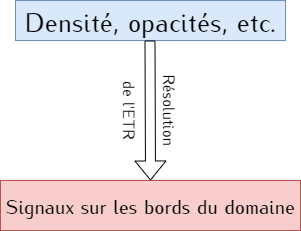
\includegraphics[width=5cm]{ProblemeDirect}       
  \end{column}
 \pause
 \begin{column}{0.5\textwidth}
    \centering
    Probleme inverse \\ (\scriptsize Reconstruction de la densite par un reseau de neurones)
    %Image de signal sur les bords -> densite
      % 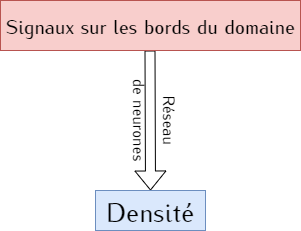
\includegraphics[width=5cm]{ProblemeInverse}       
 \end{column}
\end{columns}

\begin{figure}
  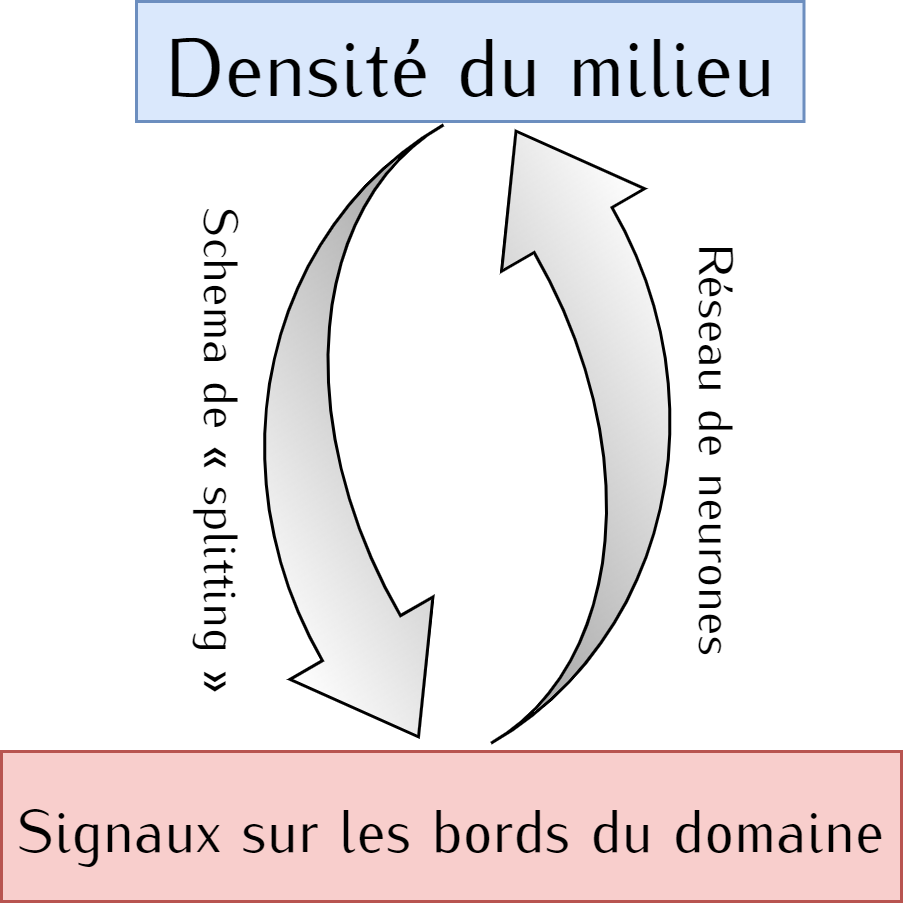
\includegraphics[width=4cm]{PBInverse}         
\end{figure}

\end{frame}
%-------- Vrai debut de l'introduction (PB INVERSE)
\begin{frame}
  \frametitle{Les point pour situer le stage}

  \begin{enumerate}
    \item Explosion du deep learning % Depuis le debut de la decenie 2010, le Machine Learning a considerablement pris de l’ampleur (2015 a l’ILSVRC, etc..)
    %%%%%% IMAGE DU DEEP LEARNING
    \item APplications dans le secteur medical (Imagerie medicale) % Avant de soigner les cancers, on doit detecter les tumeurs sont plus denses que les tissus sains (Chercher d'autres applications)
    %%%%%% IMAGE DU MEDICAL
    \item Reevaluation des methode de resolution de problemes inverse % Les problemes inverses sont difficiles. ... Les algo d'optimisation classiques marchent tres bien. En fait on s'est referer aux travaux de Maya et Guillaume Dolle. L'avantage que peuvent offrir les ANN c'est juste la simplicite, et la rapidite, et une generalisation (non specificite aux probleme)
    %%%%%% IMAGE DU PB INVERSE
  \end{enumerate}
  
\end{frame}

\begin{frame}
  \scriptsize
  \frametitle{Sommaire}
  \tableofcontents
\end{frame}


% \end{document}


% \documentclass{beamer}
% \usetheme{Szeged}

% \begin{document}


%-------------------------------------------------------------------------------
%							SECOND SECTION
%-------------------------------------------------------------------------------
\section{Principe}

\subsection{Simulation de l'ETR}

\begin{frame}
  \frametitle{Le transfer radiatif}

Lorsque la photons se trouvent en presence de la matière, Trois phenomènes majeures (caratises par leurs opacites) se produisent:

\begin{columns}
  \begin{column}{0.5\textwidth}
    \footnotesize
   \begin{itemize}
     \item Emission ($\sigma_e$): Plus la temperature matiere est elevee, plus l'emission est importante % Typiquement on ne vas pas retrouver sigma_e dans nos equations car on va se placer dans l'ETL, et on Planck.
     \item Absorption ($\sigma_a$): Lorsqu'on est a l'equilibre thermique, $\sigma_a = \sigma_e$ % On va considerer en plus l'equilibre chimique ce qui donne l'ETL
     \item Scattering ($\sigma_c$): Il faut aussi tenir compte de la fonction de distribution angulaire de "scattering" $p(\bm{\Omega^\prime \rightarrow \bm{\Omega}})$ \parencite{Reference3}.
   \end{itemize}
  \end{column}
  % \pause
  \begin{column}{0.5\textwidth}
     \begin{figure}       
      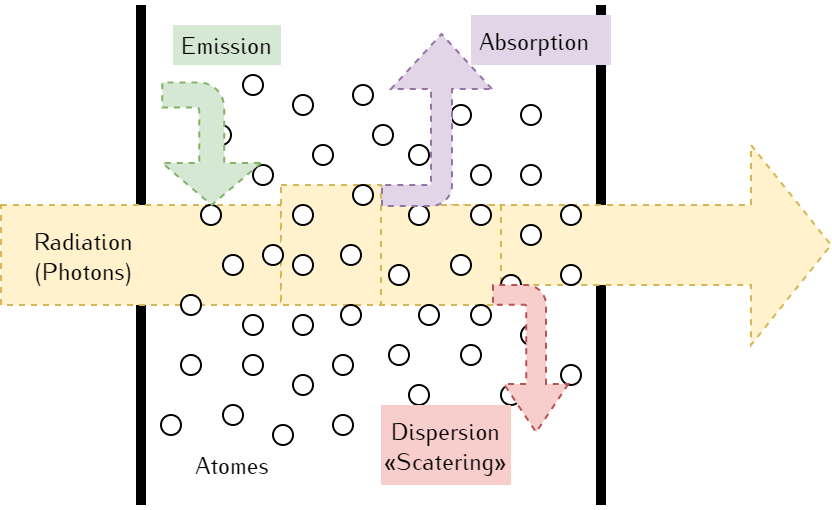
\includegraphics[width=6cm]{TransferRadiatif}       
      \caption{Interaction entre matière et radiation}
    \end{figure}
  \end{column}
 \end{columns}
 
\end{frame}

\begin{frame}
  \frametitle{L'ETR}
  L'equation du transfert radiatif est bilan d'energie lie au rayonnement au niveau mesoscopique. 

  \begingroup
  \scriptsize
  \begin{gather*}
      \begin{aligned}
      \frac{1}{c} \frac{\partial}{\partial t}I(t,\bvec{x},\bm{\Omega},\nu) &+\bm{\Omega}\cdot\nabla_{\bvec{x}} I(t,\bvec{x},\bm{\Omega},\nu) \\
      &= \sigma_a(\rho,\bm{\Omega},\nu)\left(B(\nu,T)-I(t,\bvec{x},\bm{\Omega},\nu)\right) \\
      &+ \frac{1}{4\pi} \int_{0}^{\infty} \int_{S^2}\sigma_c(\rho,\bm{\Omega},\nu)p(\bm{\Omega}^\prime\rightarrow\bm{\Omega})\left(I(t,\bvec{x},\bm{\Omega}^\prime,\nu)-I(t,\bvec{x},\bm{\Omega},\nu)\right) \, d\bm{\Omega}^\prime \, d\nu
      \end{aligned}
  % \label{eqn:ETR}
  \end{gather*}
  \endgroup
Où 
\begin{itemize}
  \item $I(t,\bvec{x},\bm{\Omega},\nu)$ designe l'intensité radiative specifique;
  \item $B(\nu,T)$ la fonction de Planck;
  \item $\oint p(\bm{\Omega}^\prime\rightarrow\bm{\Omega})\, d\bm{\Omega}^\prime=1$
\end{itemize}

\end{frame}

\begin{frame}
  \frametitle{Le modele P1}
  % Le modele P1: % Modèle macroscopique 5 aux moments (d’ordre 2), linéaire et hyperbolique. Le terme 1/3
  D'apres \parencite{Reference2}
  \begingroup
  \large
  \begin{equation*}
      \begin{cases}
       \partial_tE + c \ \operatorname {div} \bvec F = c\sigma_a\left(aT^4-E\right)\\
       \partial_t\bvec{F} + c \ \nabla E = -c\sigma_c \bvec{F} \\
       \rho C_v \partial_t T = c \sigma_a \left(E-aT^4\right)
      \end{cases}
  % \label{eqn:P1}
  \end{equation*}
  \endgroup
Ou:   % Moins precis que Monte-Carlo ou ordonne discretes; Mais plus rapide et suddisant; sigma
\begin{align*}
  E(t,\bvec{x}) &= \frac{4\pi}{c} \int_{0}^{\infty} \int_{S^2} I(t,\bvec{x},\bm{\Omega},\nu) \, d\bm{\Omega} \, d\nu \\
  \bvec{F}(t,\bvec{x}) &= \frac{4\pi}{c} \int_{0}^{\infty} \int_{S^2} \bm{\Omega}I(t,\bvec{x},\bm{\Omega},\nu) \, d\bm{\Omega} \, d\nu 
  % \label{eqn:EFT}
\end{align*}

\end{frame}

\begin{frame}
  \frametitle{Le schema de << splitting >>: Etape 1}
  % Reglage de la temperature 
  \begin{columns}
    \begin{column}{0.5\textwidth}
     A l'iteration $n$, On pose $\Theta = aT^4$

      \begingroup
      \normalsize
      \begin{equation*} 
        \begin{dcases}
         \alert<1->{E_j^{q+1} = \dfrac{\alpha E_j^n + \beta \gamma \Theta_j^n}{1 - \beta \delta}} \\
         \alert<1->{\Theta_j^{q+1} = \dfrac{\gamma \Theta_j^n + \alpha \delta E_j^n}{1 - \beta \delta}}
        \end{dcases}
    \label{eqn:Step1}
    \end{equation*}
      \endgroup
      Ou
      \tiny
      $\mu_q = \dfrac{1}{T^{3,n} + T^{n}T^{2,q} + T^{q}T^{2,n} + T^{3,q}}$
      \normalsize
    \end{column}
    % \pause
    \begin{column}{0.5\textwidth}
       \begin{center}
        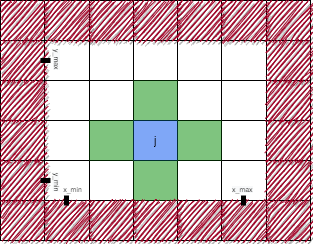
\includegraphics[width=4cm]{Dicretisation2D}       
       \end{center}
    \end{column}
   \end{columns}
   \tiny
  $\quad  \alpha = \dfrac{1}{\Delta t \left( \frac{1}{\Delta t} + c \sigma_a \right)} ,\quad 
   \beta = \dfrac{c \sigma_a}{\frac{1}{\Delta t} + c \sigma_a} ,\quad 
   \gamma = \dfrac{\rho_j C_v \mu_q}{\Delta t \left( \frac{\rho_j C_v \mu_q}{\Delta t} + c \sigma_a \right)} \quad \text{et} \quad  
   \delta = \dfrac{c \sigma_a}{\frac{\rho_j C_v \mu_q}{\Delta t} + c \sigma_a}.$

   \normalsize
   COnvergence ver $E_j^*$ et $\Theta_j^*$. $\bvec F_j$ reste constant egale a $F_j^*$.
   
\end{frame}


\begin{frame}
  \frametitle{Le schema de << splitting >>: Etape 2}   % Adaptable aussi en 2D
  \begin{columns}
    \begin{column}{0.6\textwidth}
      \begingroup
      \normalsize
      \begin{equation*} 
          \begin{dcases}
          \alert<1->{E_j^{n+1} = E_j^* + \alpha \sum_k \left( \bvec F_{jk}, \bvec n_{jk} \right)} \\
          \alert<1->{\bvec F_j^{n+1} = \beta \bvec F_j^* + \bm{\gamma} E_j^n + \delta \sum_k E_{jk} \bvec n_{jk}}
          \end{dcases}   
      % \label{eqn:Step2}
      \end{equation*}
      Avec :
      % \begingroup
      \scriptsize
    
      % \begin{gather*}    
      % \begin{aligned} 
        $\alpha = -\frac{c \Delta t}{\left| \Omega_j \right|}, \linebreak
        \beta = \frac{1}{\Delta t} \left( \frac{1}{\Delta t} + c \sum_k M_{jk} \sigma_{jk} \right)^{-1}, \linebreak
        \bm{\gamma} = \frac{c}{\left| \Omega_j \right|} \left( \frac{1}{\Delta t} + c \sum_k M_{jk} \sigma_{jk} \right)^{-1} \left( \sum_k l_{jk} M_{jk} \bvec n_{jk} \right) \linebreak
        \delta = -\frac{c}{\left| \Omega_j \right|} \left( \frac{1}{\Delta t} + c \sum_k M_{jk} \sigma_{jk} \right)^{-1}$
    %   \end{aligned}
    % \end{gather*}

    \endgroup
      
    \end{column}
    % \pause
    \begin{column}{0.4\textwidth}
      % \begin{figure}
      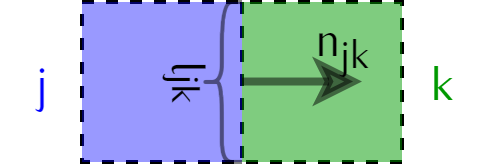
\includegraphics[width=5cm]{Interaction2D}       
        % \caption{Interaction entre deux mailles}
      % \end{figure}
       \begin{center}
        \begingroup
        \tiny
        \begin{align*}
          \left(\bvec F_{jk}, \bvec n_{jk} \right) &= l_{jk} M_{jk} \left( \frac{\bvec F_j^n \cdot \bvec n_{jk} + \bvec F_k^n \cdot \bvec n_{jk}}{2} - \frac{E_k^n - E_j^n}{2} \right) \\
          E_{jk} \bvec n_{jk} &= l_{jk} M_{jk} \left( \frac{E_j^n + E_k^n}{2} - \frac{\bvec F_k^n \cdot \bvec n_{jk} - \bvec F_j^n \cdot \bvec n_{jk}}{2} \right) \bvec n_{jk} \\
        %  \end{align*}
        %  \begin{align*}
          M_{jk} &= \frac{2}{2 + \Delta x \sigma_{jk}}  \\
          \sigma_{jk} &= \frac{1}{2} \left( \sigma_c(\rho_j,T_j^n) + \sigma_c(\rho_k,T_k^n) \right)
         \end{align*}
        \endgroup
       \end{center}
    \end{column}
   \end{columns}
\end{frame}

\begin{frame}
  \frametitle{Implementation C++}
  \begin{columns}
    \begin{column}{0.6\textwidth}
      \scriptsize
      \begin{itemize}
        \item Temps final = 0.01 \si{sh} %\textit{(1 shake (\si{sh}) = $10^{-8}$ secondes)}
        \item $c = 299$ [\si{\cm \per sh}]
        \item $a = 0.01372$ [\si{g \per cm \per sh^2  \per keV }]
        \item $C_v = 0.14361$ [\si{Jerk \per\g \per keV}] % \textit{(1 \si{Jerk} = 1\si{m \per \s\cubed})}
        \item La densité $\rho$ est un signal créneau [\si{\g\per\cm\cubed}]
        \item $\sigma_a = \rho T$ [\si{\per\cm}]
        \item $\sigma_c = \rho T$ [\si{\per\cm}]
        \item $T_0, T_{gauche} = 5$ [\si{keV}] % \textit{(en termes de température, 1 \si{keV} = 11605 \si{K})}
        \item $E_0 = aT_0^4$ [\si{g \per \cm \per sh^2}]
        \item $E_{gauche^*} = aT_{0}^4 + 5 \sin (2 k \pi t)$ [\si{g \per \cm \per sh^2}]
        \item $\bvec{F}_0, \bvec{F}_{gauche} = \bvec{0}$ [\si{g \per sh^2}]
        \item Sorties libres sur les autres bords
      \end{itemize}
    \end{column}
    % \pause
    \begin{column}{0.4\textwidth}
       \begin{figure}
        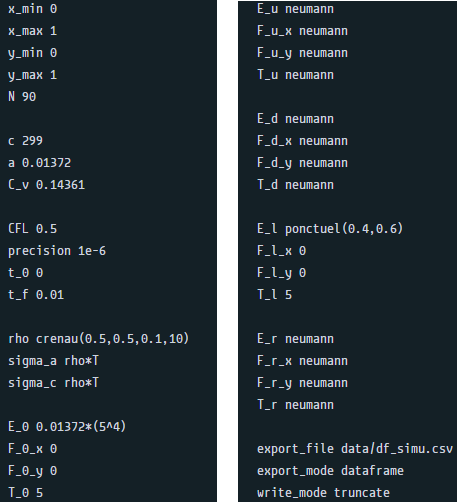
\includegraphics[width=4.5cm]{SimuCFG}   % EN 2D    
        \caption{Exemple de configuration}
      \end{figure}
    \end{column}
   \end{columns}
\end{frame}

\subsection{Reseau de neurones}

\begin{frame}
    \frametitle{L'architecture sous Keras}
    \begin{center}
        %%% Ajouter l'image des hierarchie de machine learning
        \begin{figure}
        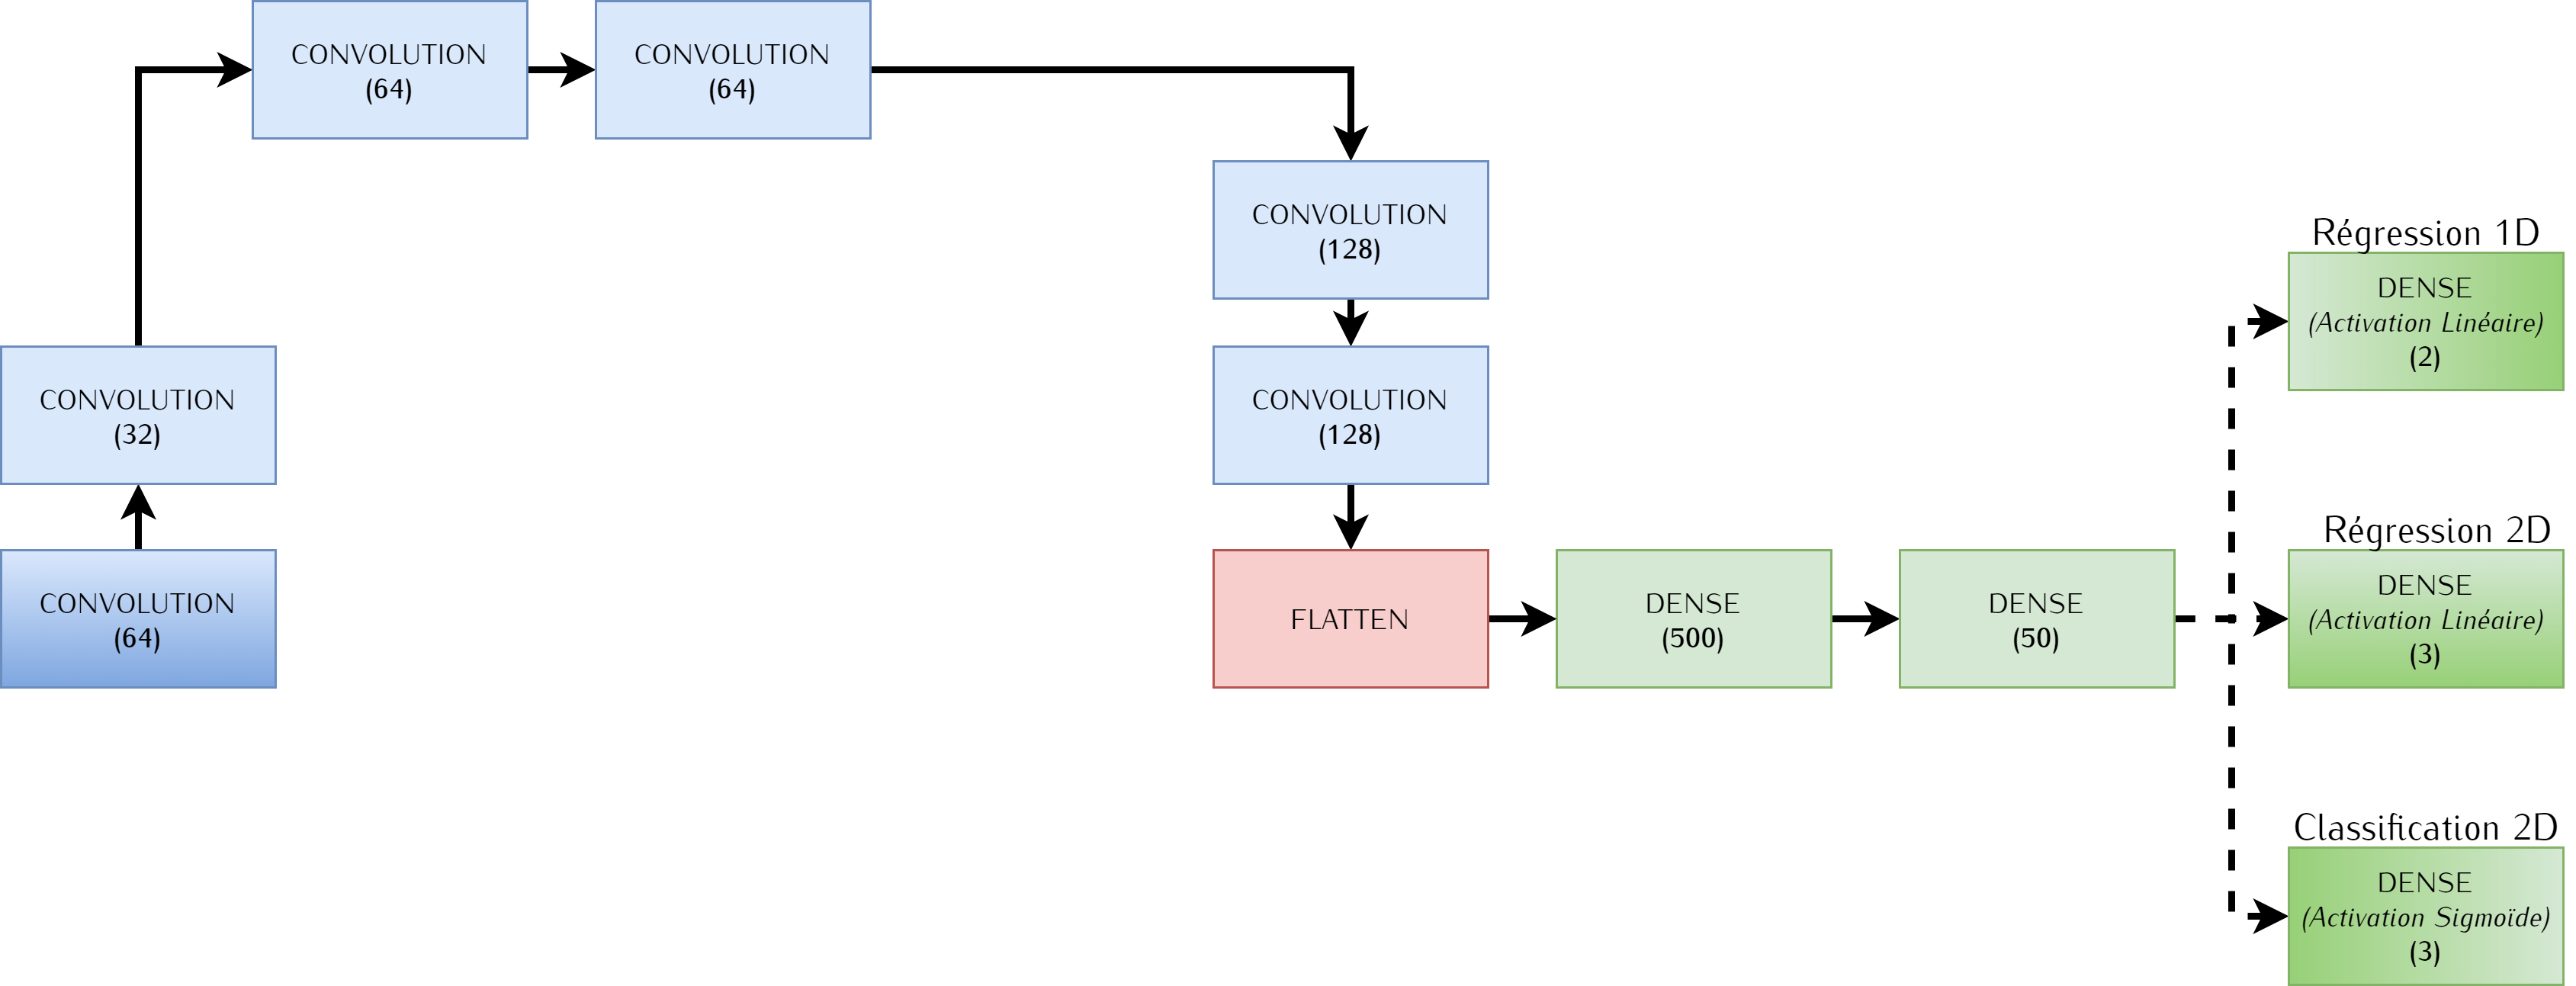
\includegraphics[width=.95\textwidth]{DRNN2}    % Modifier la sortie pour avoir 1D/Class2D/Reg 2D
        \caption{Architecture generale utilisee}
        \end{figure}
    \end{center}
\end{frame}

\begin{frame}
    \frametitle{Les couches utilisees: Convolutions (Cross-correlation)}
    \begin{columns}
        \begin{column}{0.4\textwidth}
            \scriptsize
            \begin{equation*}
                S(i) = (I * K)(i) = \sum_{m} I(i+m)K(m)
                \label{eqn:Corr2D}
            \end{equation*}
            \begin{figure}
                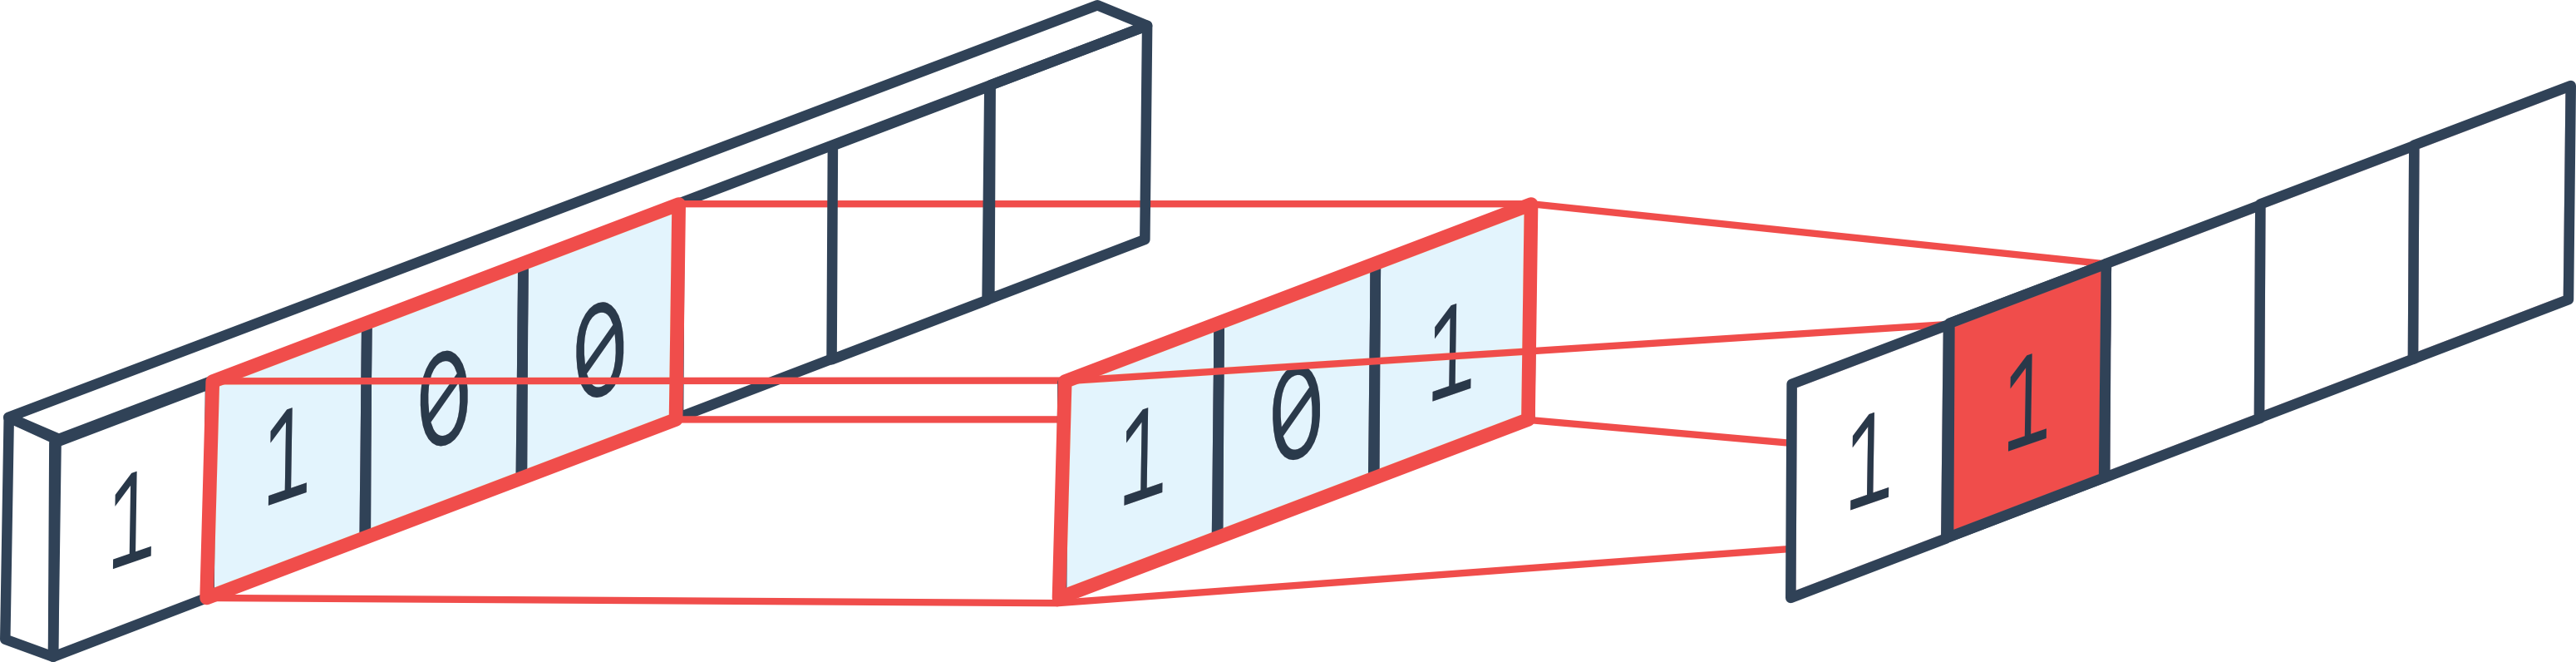
\includegraphics[width=.95\textwidth]{Conv1D}
                \caption{En 1D \parencite{Reference10}}
            \end{figure}
        \end{column}
        \begin{column}{0.6\textwidth}
            \scriptsize
            \begin{equation*}
                S(i,j) = (I * K)(i,j) = \sum_{m}\sum_{n} I(i+m,j+n)K(m,n)
                \label{eqn:Corr2D}
            \end{equation*}
            \begin{figure}
                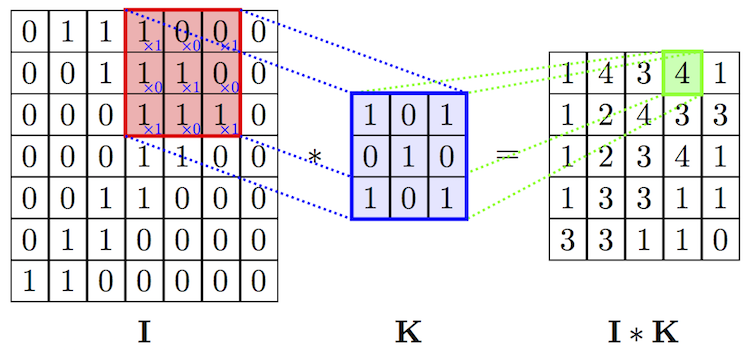
\includegraphics[width=.95\textwidth]{Conv2D}
                \caption{En 2D \parencite{Reference11}}
            \end{figure}
        \end{column}
    \end{columns}
\end{frame}

\begin{frame}
    \frametitle{Les couches utilisees: Flatten et Dense}
    \begin{columns}
        \begin{column}{0.4\textwidth}
            \begin{figure}
                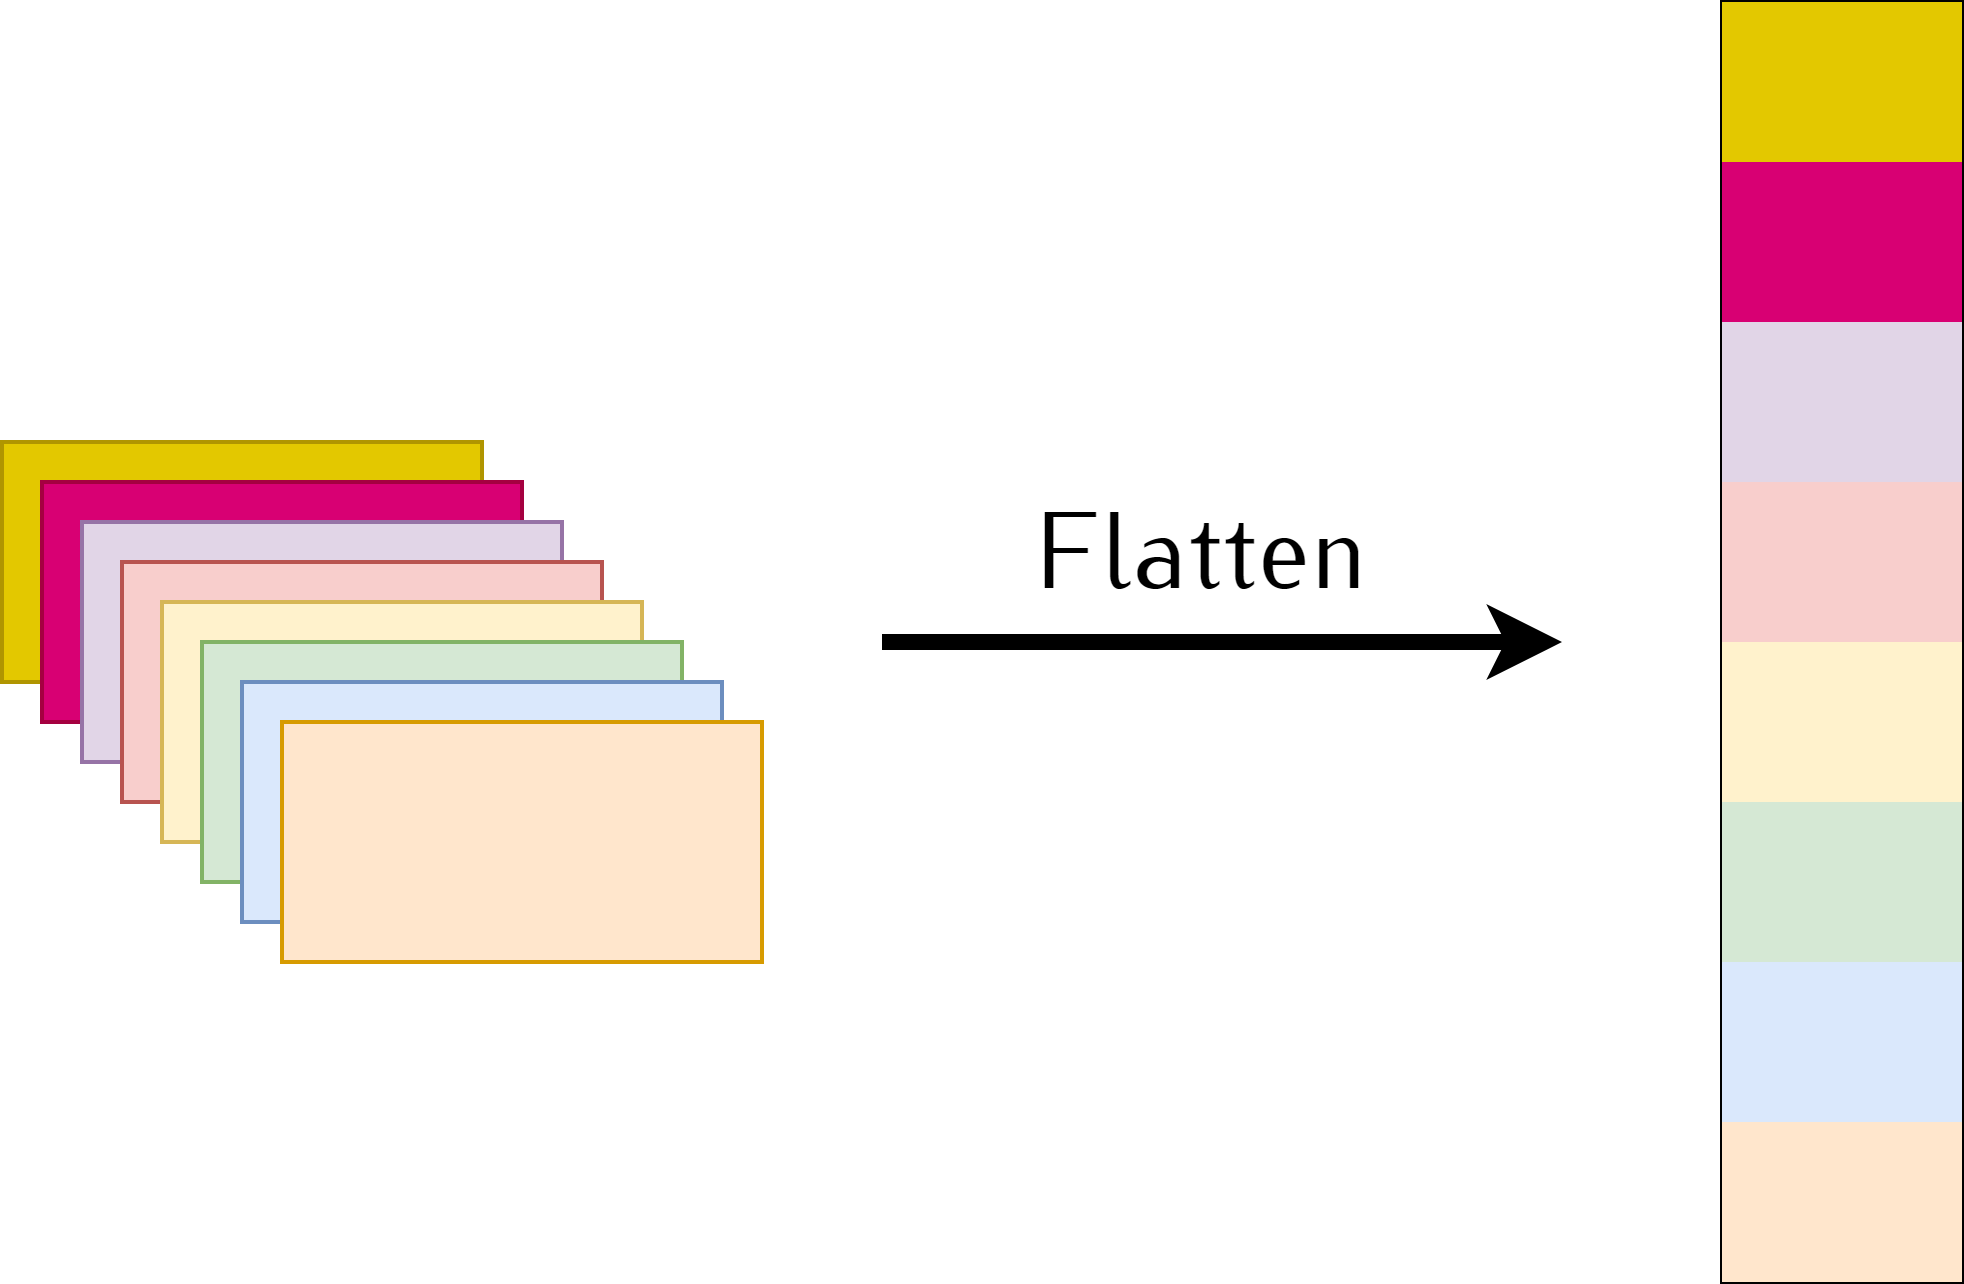
\includegraphics[width=.95\textwidth]{Flatten}
                \caption{Flatten}
            \end{figure}
        \end{column}
        \begin{column}{0.6\textwidth}
            \begin{figure}
                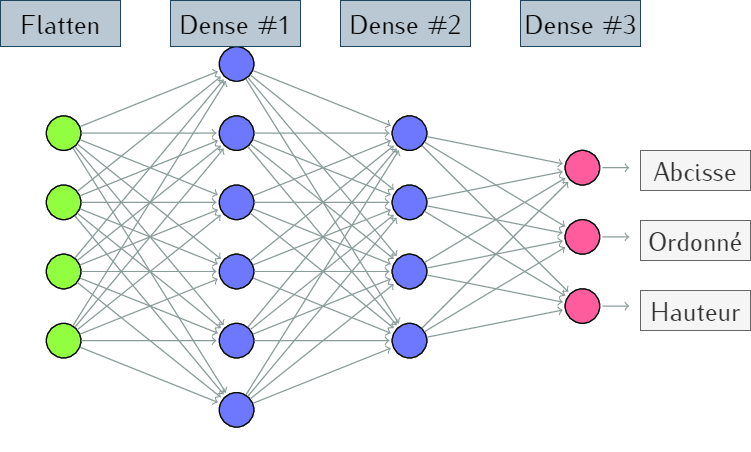
\includegraphics[width=.95\textwidth]{Dense}
                \caption{Des couches denses}
            \end{figure}
        \end{column}
    \end{columns}
\end{frame}


\begin{frame}
    \frametitle{Les metriques}
    \begin{columns}
        \begin{column}{0.5\textwidth}
            \textbf{Coefficient de determination}
        \begingroup
        \begin{align*}
            R^2 = 1 - \frac{SS_{res}}{SS_{tot}}
            \label{eqn:R2}
        \end{align*}
        Avec
        \scriptsize
        \begin{align*}
            SS_{res} &=  \sum_{i=1}^{n} \left( y_i - \hat{y}_i \right)^2 \quad \\
            SS_{tot} &=  \sum_{i=1}^{n} \left( y_i - \bar{y} \right)^2 
        \end{align*}
        Ou $ \bar{y} = \sum_{i=1}^{n} y_i $ représente la moyenne des valeurs observées.
        \endgroup
        % On peut remarquer que :
        % \begin{itemize}
        %  \item Si le modèle prédit les valeurs attendues (observées), le score $R^2$ vaut 1. 
        %  \item SI le modèle prédit toujours la valeur moyenne $\bar{y}$, le score $R^2$ vaut 0.
        %  \item Si les prédictions sont pires que la moyenne, le score $R^2$ est négatif.
        % \end{itemize}
        \end{column}
        \begin{column}{0.5\textwidth}
        \textbf{Score personalise}\\
        Pourcentage des prédiction correcte si la prediction et le label sont suffsament proche:
        \begin{itemize}
         \item \textbf{au dixième près} pour la position (suivant $x$ ou $y$) 
         \item \textbf{à l'unité près} pour la hauteur 
        \end{itemize}

        \end{column}
    \end{columns}
\end{frame}



\begin{frame}
    \frametitle{Les hyper-parametres}

    \begin{table}[h!]
        \scriptsize
        \caption{Liste des paramètres les plus influents pour l'entrainement}
        \label{tab:Parametres}
        \centering
        \begin{tabular}{l l l}
        \toprule
        \textbf{Hyper-paramètre} & \textbf{Définition} & \textbf{Valeur 1D / 2D} \\
        \midrule
        optimizer & algorithme d'optimisation & Adam\\
        learning rate & taux d'apprentissage & 1e-4 / 1e-5\\
        batch size & taille d'un batch a chaque epoque & 32\\
        epochs & nombre d'époques & 100\\
        patience & patience pour l'early stopping & 10\\
        kernel size & taille du noyau de convolution & 3 / (6,2)\\
        activation & type de fonction d'activation  & relu, linear, sigmoid\\
        \bottomrule\\
        \end{tabular}
    \end{table}

\end{frame}



% \end{document}


% \documentclass{beamer}
% \usepackage{media9}
% \usepackage{graphicx}

% \begin{document}

% \begin{frame}{Blank page}[fragile]
% Go ahead!
% \end{frame}

% La muraille de chine << text >>

% \begin{frame}[fragile]
%   \begin{center}
%     \includemedia[
%       width=0.5\linewidth,
%       activate=pageopen,
%       addresource=cube.mp4,
%       flashvars={
%          source=cube.mp4
%         &autoPlay=true
%       },
%       passcontext, % enable VPlayer's right-click menue
%     ]{\includegraphics{cubeposter.png}}{VPlayer.swf}%
%   \end{center}
% \end{frame}

% \documentclass{beamer}
% \usetheme{Szeged}

% \begin{document}

%-------------------------------------------------------------------------------
%							THIRD SECTION
%-------------------------------------------------------------------------------
\section{Resultats 1D}
Le probleme en 1D
\subsection{Simulation}

\subsection{Apprentissage}


% \end{document}



% \end{document}



% \documentclass{beamer}
% \usetheme{Szeged}

% \usepackage{media9}
% \usepackage{graphicx}

% \begin{document}

%-------------------------------------------------------------------------------
%							FOURTH SECTION
%-------------------------------------------------------------------------------
\section{Le problème en 2D}

\subsection{Simulation}

\begin{frame}[fragile]
    \frametitle{Exemple de simulation 2D}
  \begin{center}
    \includemedia[
      width=0.95\linewidth,
      activate=pageopen,
      addresource=Video2D.mp4,
      flashvars={
         source=Video2D.mp4
        &autoPlay=true
      },
      passcontext, % enable VPlayer's right-click menue
    ]{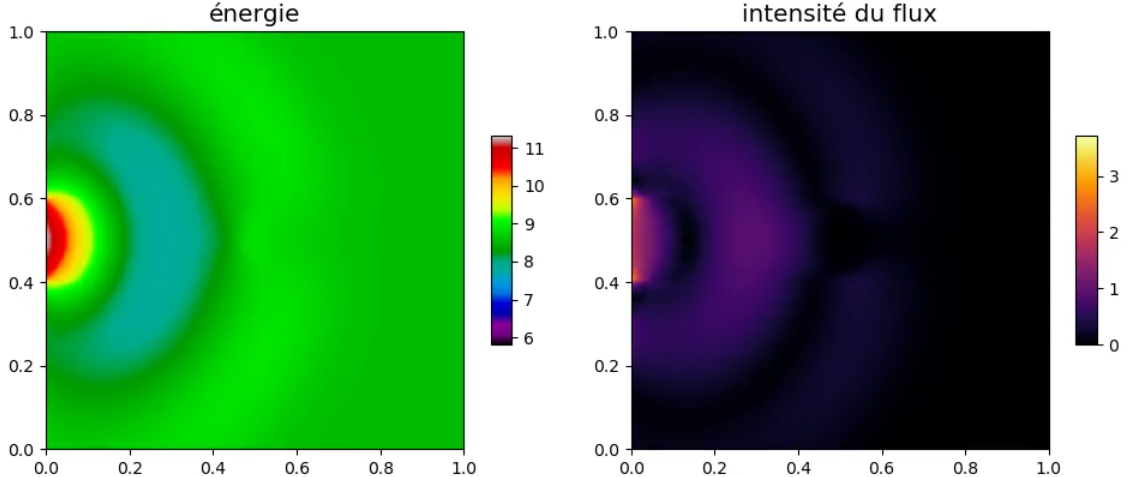
\includegraphics{Thumbnail2D.png}}{VPlayer.swf}%
  \end{center}
\end{frame}

\begin{frame}[fragile]
    \frametitle{Entrées/sorties 2D}

        \begin{figure}
        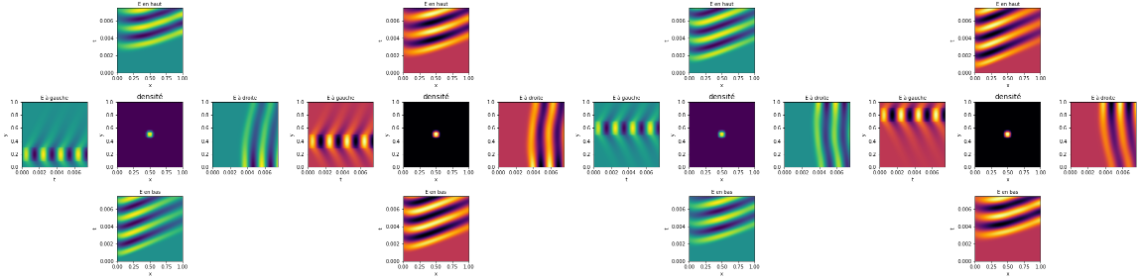
\includegraphics[width=11cm]{EntreeSortie2D}       
        \caption{Une entrée du réseau de neurones et la sortie attendue}
        \end{figure}
        \begin{figure}
        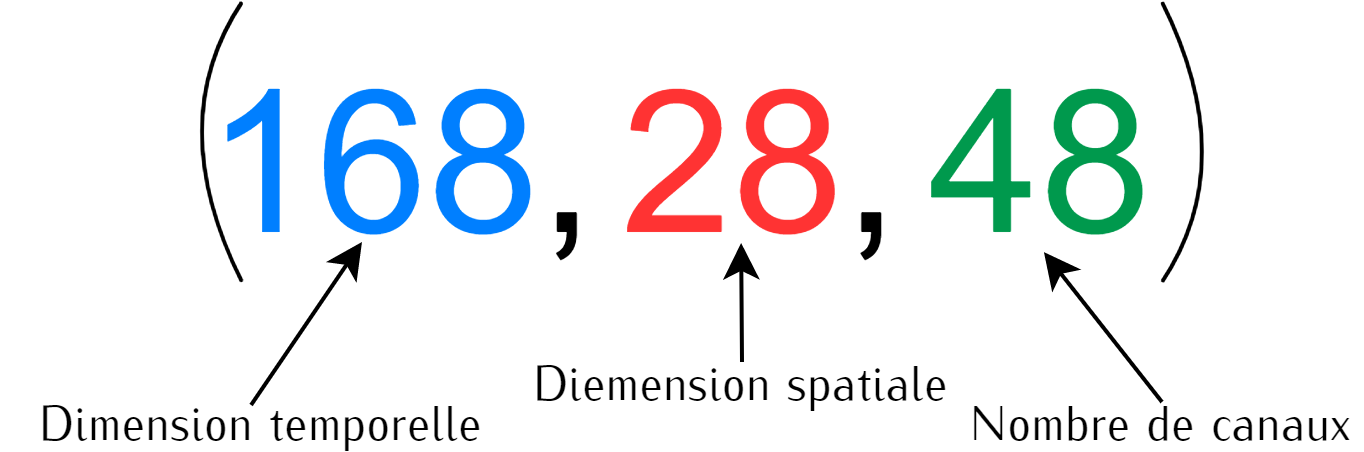
\includegraphics[width=3cm]{Entrees2D}       
        \caption{Taille d'une entrée}
        \end{figure}

\end{frame}

\subsection{Apprentissage}

\begin{frame}[fragile]
    \frametitle{Meilleures/pires prédictions du CNN}

    \begin{columns}
    \begin{column}{0.5\textwidth}
        \begin{figure}
        \includegraphics<1->[width=3cm]{Meilleur2D1}       
        \includegraphics<1->[width=3cm]{Meilleur2D2}       
        \only<1-> {\caption{Les meilleures prédictions}}
        \end{figure}
     \end{column}
     \begin{column}{0.5\textwidth}
        \begin{figure}
        \includegraphics<2>[width=2.5cm]{Pire2D1}       
        \includegraphics<2>[width=2.5cm]{Pire2D2}       
        \includegraphics<2>[width=2.5cm]{Pire2D3}       
        \only<2>{\caption{Les pires prédictions}}
        \end{figure}
     \end{column}
    \end{columns}

\end{frame}

\begin{frame}
    \frametitle{Les scores obtenus en 2D}

    \begin{table}[h!]
        \centering
        \begin{tabular}{l l}
        \toprule
        \textbf{Nom du score} & \textbf{Valeur} \\
        \midrule
        R2 & 98.81 \%\\
        Personnalisé & 93.50 \%\\
        \bottomrule\\
        \end{tabular}
    \end{table}

    \begin{columns}
        \begin{column}{0.333\textwidth}
            \begin{figure}
            \includegraphics<2->[width=2cm]{PositionX2D}       
            \only<2->{\caption{Corrélation des abscisses}}
            \end{figure}
         \end{column}
         \begin{column}{0.333\textwidth}
            \begin{figure}
            \includegraphics<3->[width=2cm]{PositionY2D}       
            \only<3->{\caption{Corrélation des ordonnées}}
            \end{figure}
         \end{column}
         \begin{column}{0.333\textwidth}
            \begin{figure}
            \includegraphics<4->[width=2cm]{Hauteur2D}       
            \only<4->{\caption{Corrélation des hauteurs}}
            \end{figure}
         \end{column}
    \end{columns}

\end{frame}


\begin{frame}
    \frametitle{Conclusion sur la régression 2D}
Détection de toutes les variables :
\begin{itemize}[<+>]
    \item L'abscisse, l'ordonnée, et la hauteur sont relativement bien prédits
    \item La valeur de la densité en dehors du créneau est connue : \textbf{reconstruction complète de la densité du milieu}
\end{itemize}
\end{frame}

\setbeamercovered{invisible}

\begin{frame}
    \frametitle{Classification 2D}
    \begin{columns}
        \begin{column}{0.7\textwidth}
            \begin{figure}
            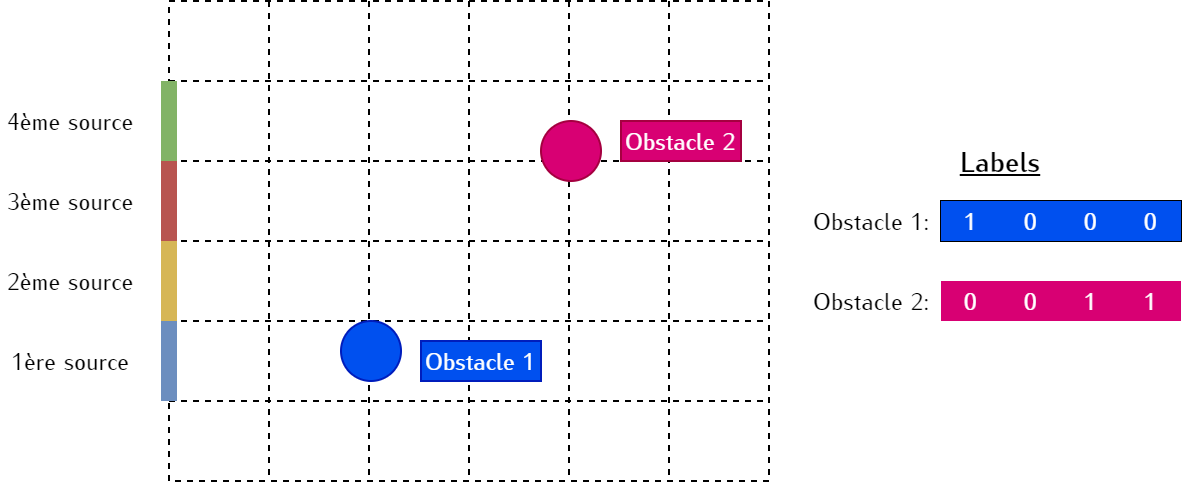
\includegraphics[width=6cm]{Classification}       
            \caption{Labels pour la classification}
            \end{figure}
         \end{column}
         \pause
         \begin{column}{0.3\textwidth}
            \begin{table}[h!]
                \caption{Les scores obtenus}
                \centering
                \begin{tabular}{l l}
                \toprule
                \textbf{Nom} & \textbf{Valeur} \\
                \midrule
                R2 & 98.86 \%\\
                Pers. & 95.45 \%\\
                \bottomrule\\
                \end{tabular}
            \end{table}
         \end{column}
    \end{columns}
\end{frame}

\setbeamercovered{transparent}

% \end{document}

% \documentclass{beamer}
% \usetheme{Szeged}

% \begin{document}

%-------------------------------------------------------------------------------
%							FITH SECTION
%-------------------------------------------------------------------------------


\section{Conclusion}
% Conclusion

\subsection{Sur l'apprentissage}
\begin{frame}
    \frametitle{Bilan de l'apprentissage}
    \begin{enumerate}
        \item \textbf{Régression 1D} : Permet de détecter la hauteur du créneau %sur la densité d'un domaine 1D (avec la meilleure corrélation de tous les apprentissages). Elle n'a cependant pas été capable de détecter la position du créneau, probablement dû au caractère mal posé du problème inverse.
        \item \textbf{Classification 2D} : Permet de localiser l'ordonnée du créneau %en le situant par rapport aux sources sur la gauche d'un domaine 2D. En augmentant leur nombre et en plaçant certaines sources en haut (ou en bas) du domaine, on pourrait localiser avec plus de finesse l'abscisse et l'ordonnée du créneau.
        \item \textbf{Régression 2D} : Permet de prédire tous les attributs essentiels du créneau (abscisse, ordonnée, et hauteur)%, tout ceci avec une très forte précision (score personnalisé s'élevant à 93 \%). 
      \end{enumerate}
\end{frame}

\subsection{Generale}
\begin{frame}
    \frametitle{Bilan du stage}
    \begin{figure}
        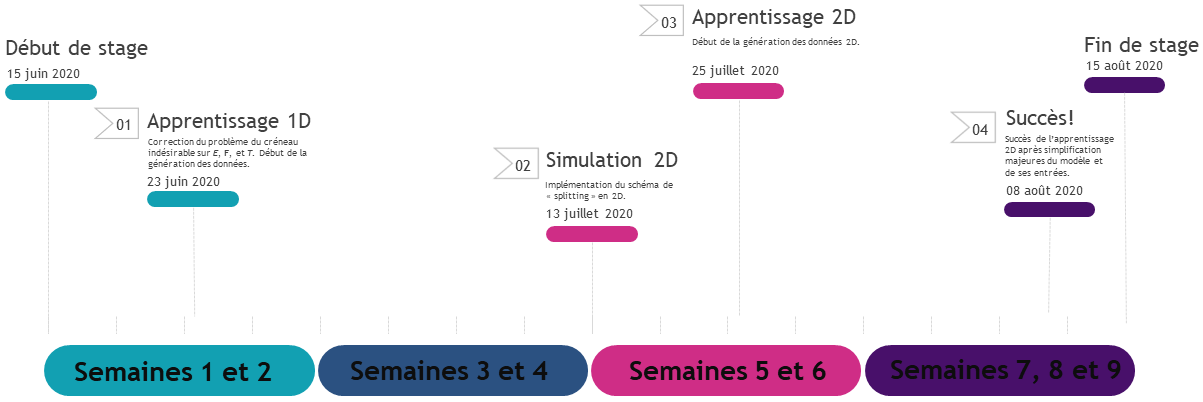
\includegraphics[width=10cm]{MilestonesRoadmap}       
        \caption{Points tournants du le stage}
    \end{figure}
\end{frame}

\begin{frame}
    \frametitle{Apports et enseignements}
    \begin{itemize}
        \item Developpement C++ et Python   % Mettre en pratique les connaissances de CSMI
        \item Equations aux derivees partielles % technique de verification
        \item Reseaux de neurones % (Keras, Tensorflow, learning rate)
        \item Experience dans un milieu de recherche % J'ai apprecieer travailler sur IA+EDP
        % \item Point negatif: Manque de coordination (A cause du COVID)
    \end{itemize}
\end{frame}


% \end{document}


% %-------------------------------------------------------------------------------
% %							THE BIBLIOGRAPHY
% %-------------------------------------------------------------------------------
\appendix   % Pour retirer les references de la bare de navigation
\printbibliography

\end{document}
